\documentclass[11pt,a4paper]{article}

%==============================================================================
% Fonts & Typography
%==============================================================================
\usepackage[T1]{fontenc}
\usepackage{lmodern}
\usepackage{microtype}

%==============================================================================
% Core Packages
%==============================================================================
\usepackage{graphicx}
\usepackage{geometry}
\usepackage{hyperref}
\usepackage{enumitem}
\usepackage{booktabs}
\usepackage{xcolor}
\usepackage{tikz}
\usepackage{float}
\usepackage{fancyhdr}
\usepackage{tabularx}
\usepackage{amssymb}
\usepackage{multicol}
\usepackage{titlesec}

\usetikzlibrary{shapes.geometric, arrows, positioning, fit, backgrounds}

%==============================================================================
% Page Geometry
%==============================================================================
\geometry{
  margin=0.85in,
  top=0.75in,
  bottom=0.75in
}

%==============================================================================
% Color Palette
%==============================================================================
\definecolor{primary}{HTML}{1F4FD8}
\definecolor{secondary}{HTML}{F59E0B}
\definecolor{success}{HTML}{10B981}
\definecolor{danger}{HTML}{EF4444}
\definecolor{muted}{HTML}{6B7280}

\hypersetup{
  colorlinks=true,
  linkcolor=primary,
  urlcolor=primary
}

%==============================================================================
% Section Styling
%==============================================================================
\titleformat{\section}
  {\Large\bfseries\color{primary}}
  {}
  {0pt}
  {}

\titleformat{\subsection}
  {\large\bfseries\color{secondary}}
  {}
  {0pt}
  {}

\titlespacing*{\section}{0pt}{1.2em}{0.6em}

%==============================================================================
% Lists
%==============================================================================
\setlist[itemize]{noitemsep, topsep=4pt, leftmargin=*}
\setlist[enumerate]{noitemsep, topsep=4pt, leftmargin=*}

%==============================================================================
% Header / Footer
%==============================================================================
\pagestyle{fancy}
\fancyhf{}
\lhead{\textbf{Youness Anouar}}
\rhead{\textcolor{muted}{Binary Analysis Agent}}
\rfoot{\textcolor{muted}{\thepage}}
\renewcommand{\headrulewidth}{0.3pt}
\renewcommand{\footrulewidth}{0pt}

%==============================================================================
% Title
%==============================================================================
\title{
  \vspace{-1.5cm}
  \textbf{\Huge Agentic Workflow for Automated Binary Analysis}\\
  \vspace{0.3em}
  \Large\textcolor{muted}{Project Plan}
}
\author{Youness Anouar}
\date{\today}

\begin{document}
\maketitle
\vspace{-0.8cm}

%==============================================================================
\section{Project Overview}
%==============================================================================

\noindent\textbf{Duration:} 8 weeks \\ \textbf{Repository:} \url{https://github.com/Uness10/Agentic-Workflow-for-Automated-Binary-Analysis}

\vspace{0.4em}
\noindent AI-powered system that automates security analysis of PE (.exe) and ELF binaries using LLM-orchestrated specialized tools built with the \textbf{Agno} framework and \textbf{FastMCP} servers.

\vspace{0.4em}
\noindent\textbf{Objectives:}
\begin{enumerate}
  \item Design and implement high-level analysis tools as MCP servers
  \item Build intelligent agent orchestration for automated workflows
  \item Detect malicious patterns, obfuscation, and suspicious behaviors
  \item Generate comprehensive security reports with actionable insights
  \item Package the entire system as reproducible Docker containers
\end{enumerate}

%==============================================================================
\section{Methodology}
%==============================================================================

\subsection{High-Level Approach}
The system follows a \textbf{modular, agent-driven architecture} using the ReAct (Reasoning + Acting) paradigm:

\begin{enumerate}
  \item \textbf{Input Processing:} Binary files (.exe/.elf) are submitted and validated (format detection, size checks)
  \item \textbf{Reasoning:} The LLM-based agent analyzes the binary type and determines the optimal analysis strategy
  \item \textbf{Tool Selection:} Agent dynamically selects which MCP tools to invoke based on context and intermediate findings
  \item \textbf{Specialized Analysis:} Each MCP server performs focused, high-level analysis (semantic, not raw commands)
  \item \textbf{Result Correlation:} Findings from multiple tools are aggregated, cross-referenced, and synthesized
  \item \textbf{Report Generation:} A structured security report is produced with severity ratings and recommendations
\end{enumerate}

\noindent The agent operates in an iterative loop—if initial analysis reveals suspicious patterns (e.g., packing detected), it triggers deeper investigation with additional tools.

\subsection{System Architecture Diagram}

\begin{figure}[H]
\centering
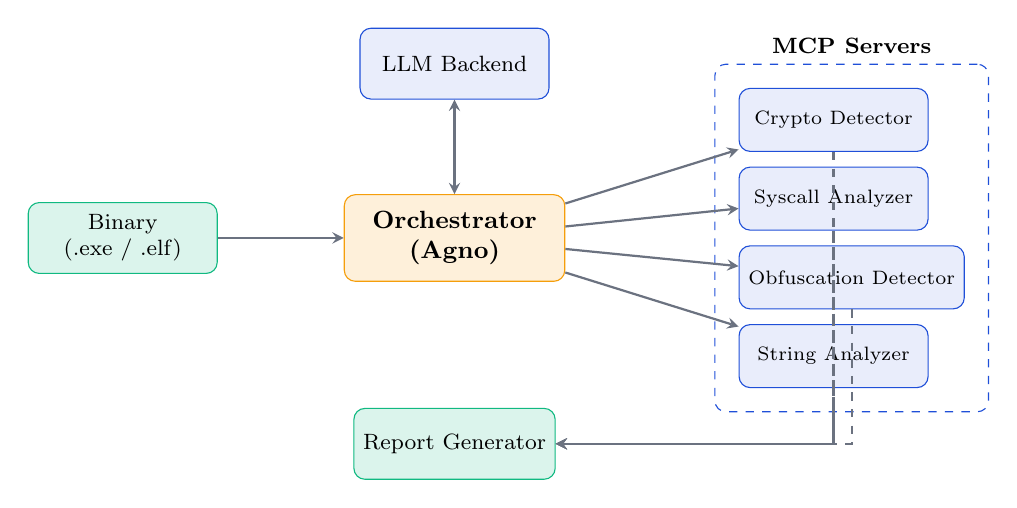
\begin{tikzpicture}[
    node distance=1cm and 1.4cm,
    box/.style={rectangle, draw=success, rounded corners, minimum width=2.4cm, minimum height=0.9cm, align=center, fill=success!15, font=\footnotesize},
    mcpbox/.style={rectangle, draw=primary, rounded corners, minimum width=2.4cm, minimum height=0.8cm, align=center, fill=primary!10, font=\scriptsize},
    agent/.style={rectangle, draw=secondary, rounded corners, minimum width=2.8cm, minimum height=1.1cm, align=center, fill=secondary!15, font=\small\bfseries},
    arrow/.style={->, thick, color=muted, >=stealth}
]
\node[box] (input) {Binary\\(.exe / .elf)};
\node[agent, right=1.6cm of input] (orchestrator) {Orchestrator\\(Agno)};
\node[mcpbox, right=2.2cm of orchestrator, yshift=1.5cm] (crypto) {Crypto Detector};
\node[mcpbox, right=2.2cm of orchestrator, yshift=0.5cm] (syscall) {Syscall Analyzer};
\node[mcpbox, right=2.2cm of orchestrator, yshift=-0.5cm] (obfuscation) {Obfuscation Detector};
\node[mcpbox, right=2.2cm of orchestrator, yshift=-1.5cm] (strings) {String Analyzer};
\node[box, below=1.6cm of orchestrator] (report) {Report Generator};
\node[box, above=1.2cm of orchestrator, fill=primary!10, draw=primary] (llm) {LLM Backend};
\draw[arrow] (input) -- (orchestrator);
\draw[arrow] (orchestrator) -- (crypto);
\draw[arrow] (orchestrator) -- (syscall);
\draw[arrow] (orchestrator) -- (obfuscation);
\draw[arrow] (orchestrator) -- (strings);
\draw[arrow, dashed] (crypto) |- (report);
\draw[arrow, dashed] (syscall) |- (report);
\draw[arrow, dashed] (obfuscation) |- (report);
\draw[arrow, dashed] (strings) |- (report);
\draw[arrow, <->] (orchestrator) -- (llm);
\begin{scope}[on background layer]
  \node[fit=(crypto)(syscall)(obfuscation)(strings), draw=primary, dashed, rounded corners, inner sep=0.3cm, label=above:{\footnotesize\textbf{MCP Servers}}] {};
\end{scope}
\end{tikzpicture}
\vspace{-0.3cm}
\caption{System Architecture — Agent orchestrates MCP tools via LLM reasoning}
\end{figure}

\subsection{Key Components and Interactions}

\begin{table}[H]
\centering\small
\begin{tabularx}{\textwidth}{l X}
\toprule
\textbf{Component} & \textbf{Role \& Interactions} \\
\midrule
\textbf{Orchestrator Agent} & Central coordinator (Agno framework). Receives binary input, queries LLM for reasoning, invokes MCP tools, aggregates results. Implements ReAct loop for iterative analysis. \\
\textbf{LLM Backend} & Provides reasoning capabilities. Agent sends context (binary metadata, partial findings) and receives tool selection decisions and analysis interpretations. \\
\textbf{MCP Tool Servers} & Five specialized analyzers exposed via FastMCP protocol. Each tool is stateless, accepts file path, returns structured JSON. Tools can be invoked in parallel or sequentially. \\
\textbf{Report Generator} & Consumes aggregated tool outputs. Applies severity scoring, generates Markdown/JSON reports with MITRE ATT\&CK mappings and remediation suggestions. \\
\bottomrule
\end{tabularx}
\end{table}

\subsection{Technology Stack Justification}

\begin{table}[H]
\centering\small
\begin{tabularx}{\textwidth}{l l X}
\toprule
\textbf{Layer} & \textbf{Technology} & \textbf{Justification} \\
\midrule
Agent Framework & Agno & Modern Python framework with native tool orchestration, async support, and clean agent abstractions. Preferred over LangChain for simplicity. \\
Tool Protocol & FastMCP & Lightweight Model Context Protocol implementation. Enables clean tool exposure to LLM agents with structured I/O schemas. \\
Binary Analysis & Radare2, LIEF & Radare2: mature RE framework for deep analysis. LIEF: cross-platform binary parsing (PE/ELF/Mach-O) with Python bindings. \\
PE/ELF Parsing & pefile, pyelftools & Specialized libraries for header parsing, import tables, sections. More reliable than generic parsers for format-specific details. \\
LLM & OpenAI / Claude & State-of-the-art reasoning capabilities. Claude preferred for longer context; OpenAI for function calling reliability. \\
Containerization & Docker & Ensures reproducibility across environments. Critical for packaging complex dependencies (Radare2, native libs). \\
\bottomrule
\end{tabularx}
\end{table}

%==============================================================================
\section{MCP Tools Specification}
%==============================================================================

\noindent Tools are \textbf{high-level semantic analyzers} (not command wrappers). Each accepts a binary path and returns structured JSON.

\vspace{0.4em}
\begin{multicols}{2}

\noindent\textbf{1. Crypto Detector}
\begin{itemize}
  \item Identifies cryptographic constants (AES, RC4, RSA)
  \item Detects custom encryption patterns
  \item Returns: algorithm, confidence, location
\end{itemize}

\noindent\textbf{2. Syscall Analyzer}
\begin{itemize}
  \item Maps imports to MITRE ATT\&CK
  \item Detects suspicious API combinations
  \item Returns: behaviors, risk score, techniques
\end{itemize}

\columnbreak

\noindent\textbf{3. Obfuscation Detector}
\begin{itemize}
  \item Identifies packers (UPX, etc.)
  \item Analyzes entropy anomalies
  \item Returns: packer ID, evasion score
\end{itemize}

\noindent\textbf{4. String Analyzer}
\begin{itemize}
  \item Extracts contextual strings
  \item Categorizes URLs, IPs, and commands
  \item Returns: categorized strings, risk flags
\end{itemize}

\end{multicols}

\vspace{0.2cm}
\noindent\textbf{5. Metadata Extractor} — Parses PE/ELF headers; extracts timestamps, compiler info, signatures, and flags anomalies.

%==============================================================================
\section{Implementation Plan}
%==============================================================================

\subsection{Timeline with Milestones}

\begin{table}[H]
\centering\small
\begin{tabularx}{\textwidth}{c l X}
\toprule
\textbf{Weeks} & \textbf{Milestone} & \textbf{Deliverables} \\
\midrule
1--2 & Foundation & Repository structure, Dockerfile, FastMCP template, Agno skeleton, data models \\
3--4 & Core Tools & Crypto, String, Syscall, Metadata MCP servers + unit tests \\
5--6 & Orchestration & Obfuscation MCP, agent workflow, tool coordination, error handling \\
7--8 & Delivery & Report generator, E2E testing, documentation, Docker Compose, demo \\
\bottomrule
\end{tabularx}
\end{table}

\subsection{Task Breakdown and Assignments}

\noindent\textbf{Milestone 1 (Weeks 1--2): Foundation \& Infrastructure}
\begin{itemize}
  \item Initialize Git repository with modular structure (\texttt{/agents}, \texttt{/tools}, \texttt{/core})
  \item Create base Dockerfile with dependencies (Radare2, pefile, pyelftools, LIEF)
  \item Implement FastMCP server boilerplate with JSON schema definitions
  \item Build Agno agent skeleton with tool registration mechanism
  \item Design common data models: \texttt{BinaryInfo}, \texttt{AnalysisResult}, \texttt{Finding}
  \item Implement binary utilities: format detection (PE/ELF), file validation, hash computation
\end{itemize}

\noindent\textbf{Milestone 2 (Weeks 3--4): Core MCP Tools}
\begin{itemize}
  \item Implement Crypto Detector: constant scanning, entropy-based detection, algorithm identification
  \item Implement String Analyzer: extraction, regex categorization, context retrieval
  \item Implement Syscall Analyzer: import table parsing, API-to-ATT\&CK mapping, risk scoring
  \item Implement Metadata Extractor: header parsing, timestamp analysis, anomaly detection
  \item Write unit tests for each tool (pytest); validate with benign and malicious samples
\end{itemize}

\noindent\textbf{Milestone 3 (Weeks 5--6): Advanced Tools \& Orchestration}
\begin{itemize}
  \item Implement Obfuscation Detector: packer signatures, entropy analysis, anti-debug checks
  \item Integrate all MCP tools with Agno agent via FastMCP protocol
  \item Define agent system prompts and ReAct decision logic
  \item Implement tool selection strategy (parallel vs. sequential based on findings)
  \item Add result correlation: cross-reference findings, deduplicate, compute aggregate risk
  \item Handle errors: timeouts, malformed binaries, LLM failures with graceful fallbacks
\end{itemize}

\noindent\textbf{Milestone 4 (Weeks 7--8): Integration \& Delivery}
\begin{itemize}
  \item Design report schema: JSON for programmatic use, Markdown for human readability
  \item Implement severity scoring: weighted combination of tool findings
  \item Perform end-to-end integration testing with diverse binary corpus
  \item Finalize \texttt{docker-compose.yml} for multi-container orchestration
  \item Write \texttt{start.sh}: environment variable checks, dependency validation, service startup
  \item Complete documentation: README, API reference, usage tutorials, architecture diagrams
  \item Prepare demo: analyze sample malware, generate reports, record walkthrough
\end{itemize}

\subsection{Dependencies and Risk Mitigation}

\begin{table}[H]
\centering\small
\begin{tabularx}{\textwidth}{l l X}
\toprule
\textbf{Risk} & \textbf{Impact} & \textbf{Mitigation Strategy} \\
\midrule
LLM API rate limits & Workflow interruption & Implement response caching, exponential retry, local LLM fallback (Ollama) \\
Binary parsing failures & Tool crashes & Use multiple parsers (pefile + LIEF) with fallback chain; validate inputs \\
Large binary analysis & Timeouts, OOM & Chunked processing, configurable timeouts, memory limits in Docker \\
False positives/negatives & Inaccurate reports & Calibrate detection thresholds, ensemble scoring, confidence intervals \\
Docker build failures & Deployment blocked & Pin all dependency versions, use multi-stage builds, CI/CD validation \\
\bottomrule
\end{tabularx}
\end{table}

%==============================================================================
\section{Deliverables \& Success Criteria}
%==============================================================================

\begin{multicols}{2}

\noindent\textbf{Deliverables}
\begin{itemize}
  \item Python codebase and test suite
  \item Dockerfile and docker-compose.yml
  \item start.sh with environment validation
  \item README, API docs, tutorials
  \item Demo analysis reports
\end{itemize}

\columnbreak

\noindent\textbf{Success Criteria}
\begin{itemize}
  \item[$\square$] Five MCP tools fully functional
  \item[$\square$] Agent orchestrates multi-tool analysis
  \item[$\square$] Supports PE and ELF binaries
  \item[$\square$] Docker runs without intervention
  \item[$\square$] Reports contain actionable findings
\end{itemize}

\end{multicols}

%==============================================================================
\section{Important Notes}
%==============================================================================

The system architecture, technology stack, and project milestones are intended as a reference plan.  
They may be adjusted or refined as the project evolves to address new findings, integration challenges, or performance optimizations.  
All modifications will maintain the modular agent–MCP design and the principle of reproducible, containerized deployment.

\end{document}
